\documentclass[12pt,a4paper]{article}
\usepackage[utf8x]{inputenc}
\usepackage[french]{babel}
\usepackage[T1]{fontenc}
\usepackage{amsmath}
\usepackage{amsfonts}
\usepackage{amssymb}
\usepackage{graphicx}
\usepackage{url}
\usepackage[usenames,dvipsnames]{xcolor}
\usepackage[colorlinks=false,urlbordercolor=white,linkbordercolor=white]{hyperref}
\usepackage[left=2cm,right=2cm,top=2cm,bottom=3cm]{geometry}
\usepackage{fancyhdr}
\usepackage{lmodern}
\usepackage{listings}
\pagestyle{fancy}
\usepackage{titlesec}
\usepackage[abs]{overpic}
\usepackage{tabularx}
\usepackage{times}
% gestion de la police sans-serif (helvetica, équivalent arial) :
% décommenter les deux lignes suivantes
%\usepackage{helvet}
%\renewcommand{\familydefault}{\sfdefault}

% Definition de l'affichage du code
\lstset{breaklines=true
,basicstyle=\footnotesize\ttfamily
,frame=none
, numbers=none
%,backgroundcolor=\color{lightgray}
}

% Definition des couleurs
\definecolor{titreColor}{RGB}{0,58,128}  % Marine
\definecolor{stitreColor}{RGB}{0,158,224}  % Ocean
\definecolor{auteurColor}{RGB}{0,58,128}     % Marine
\definecolor{texteColor}{RGB}{164,196,0}     % Prairie

% Definition du sommaire
\usepackage[tight]{shorttoc}
\newcommand{\sommaire}{\shorttoc{Sommaire}{2}}

% Definition des chapitres
\titleformat{\section}
{\color{titreColor}\normalfont\Large\bfseries\sffamily}
{\color{titreColor}\thesection}{1em}{}

\titleformat{\subsection}
{\color{stitreColor}\bfseries\sffamily}
{\color{stitreColor}\thesubsection}{1em}{}

%Données de titre et d'auteur pour la page de garde
\newcommand{\titre}{SHOMIMPORT -- Coefficients de marée}
\newcommand{\sousTitre}{Utilitaire d'extraction des coefficients de marées fournis par le SHOM pour importation dans une base de données}
\newcommand{\auteur}{Éric Quinton}
\newcommand{\dateModif}{\today}

\begin{document}
%Supprime les veuves et orphelines
\widowpenalty=10000
\clubpenalty=10000
\raggedbottom 

%entete
\fancyhead{}
\renewcommand{\headrulewidth}{0pt}
%pied de page
\fancyfoot{}
\fancyfoot[C]{\sffamily\thepage}
\fancyfoot[L]{\textcolor{titreColor}{\sffamily\textbf{IRSTEA} - Centre de Bordeaux\\}
\fancyfoot[R]{\textcolor{auteurColor}{\sffamily\auteur{}}\\{\sffamily\dateModif{}}}
\textcolor{stitreColor}{\sffamily 50, avenue de Verdun, Gazinet\\
33612 CESTAS Cedex }}
\fancyfoot[R]{\sffamily\author{}}

% Insertion du logo, du titre et du sous-titre
\begin{minipage}{0.2\linewidth}

\includegraphics[width=3.06cm,height=9.57cm,keepaspectratio]{logo_irstea}%
\end{minipage}
\hspace{0.1cm}
\begin{minipage}{0.8\linewidth}
\LARGE\flushleft \color{titreColor}{\bfseries\sffamily\titre{}}\\
\large\flushleft \color{stitreColor}{\bfseries\sffamily\sousTitre{}}
\end{minipage}

% Insertion du sommaire
% \sommaire
%\tableofcontents

% Debut effectif du texte
\section{Présentation}

Le logiciel SHOMIMPORT permet d'importer les fichiers fournis par le SHOM, et contenant les coefficients de marée pour une station, dans une base de données. Le programme a été écrit pour fonctionner avec une base de données PostgreSQL, mais il devrait pouvoir être facilement adapté à MySQL.

\section{Installation de PHP}
Le logiciel fonctionne en ligne de commande, et utilise PHP comme interpréteur.

\subsection{Installation Linux}
Installez PHP avec la commande :
\begin{lstlisting}
sudo apt install php7.2-cli php7.2-mbstring php7.2-pgsql
\end{lstlisting}

Vérifiez, dans le fichier de configuration (/etc/php/7.2/cli/php.ini), que le composant \textit{mbstring} est bien activé :
\begin{lstlisting}
extension=mbstring
\end{lstlisting}


\subsection{Installation Windows}
Téléchargez la version PHP \textit{Non Thread Safe} depuis le site de PHP : \href{https://windows.php.net/download/}{https://windows.php.net/download/}.

\section{Installation du code}
Téléchargez le code depuis Github : \href{https://github.com/Irstea/magest/archive/master.zip}{https://github.com/Irstea/magest/archive/master.zip}

Décompressez l'archive dans votre arborescence. Renommez le dossier \textit{shomimport-master} en \textit{shomimport}.

Renommez le fichier \textit{param-dist.ini} en \textit{param.ini}.

S'ils n'existent pas, créez les dossiers \textit{shomimport/import} et \textit{shomimport/treated}, qui seront utilisés pour déposer les fichiers à traiter ou traités.

\subsection{Tester l'installation}

Linux :
\begin{itemize}
\item ouvrez un terminal, et positionnez-vous dans le dossier \textit{magest}
\item lancez la commande :
\begin{lstlisting}
php shomimport.php -h
\end{lstlisting}
pour afficher le message d'aide.
\end{itemize}

Windows 10 :
\begin{itemize}
\item Ouvrez un terminal \textit{PowerShell} (dans le menu, \textit{Windows PowerShell > Windows PowerShell}). Si \textit{Windows PowerShell} n'est pas installé (ce qui est possible), installez-le depuis le centre de gestion des logiciels de Windows.
\item Positionnez vous dans le sous-dossier \textit{magest} :
\begin{lstlisting}
cd .\Documents\magest
\end{lstlisting}
\item lancez la commande :
\begin{lstlisting}
../php/php.exe shomimport.php -h
\end{lstlisting}
pour afficher le message d'aide.
\end{itemize}
. 

\section{Paramétrage}
Les paramètres utilisés pour faire fonctionner le script sont décrits dans le fichier \textit{param.ini}.

Attention : avec une machine Windows, le fichier ne doit être édité qu'avec Notepad++ (\url{https://notepad-plus-plus.org}), en raison de l'encodage des fins de lignes qui ne sont pas identiques entre Linux et Windows.

Les paramètres sont organisés par section :

\subsection{general}
L'ensemble des paramètres de cette section peuvent être modifiés en ligne de commande.

% \usepackage{array} is required
\begin{tabular}{|l|>{\raggedright\arraybackslash}p{12cm}|}
\hline 
attribut & Signification \\ 
\hline 
source & dossier contenant les fichiers à traiter  \\ 
treated & dossier où les dossiers traités sont déplacés en fin de traitement \\ 
dsn & paramètres de connexion à la base de données, en suivant les prescriptions de PHP PDO (\textit{cf.} \href{https://www.php.net/manual/fr/pdo.construct.php}{https://www.php.net/manual/fr/pdo.construct.php}) \\ 
schema &  Nom du schéma contenant la table à alimenter\\ 
login & Nom du compte utilisé pour se connecter à la base de données \\ 
password & Mot de passe associé au login \\ 
filetype & extension des fichiers contenant les données \\
\hline 
\end{tabular} 

\subsection{Station}

Une section par station doit être créée. Elle contient les informations de correction d'heure et de hauteur d'eau pour une station, par rapport aux données de référence fournies.

\begin{tabular}{|l|>{\raggedright\arraybackslash}p{12cm}|}
\hline 
attribut & Signification \\ 
\hline 
pmheure95 & Décalage en minutes de l'heure de pleine mer à coefficient 95 \\
pmheure45 & Décalage en minutes de l'heure de pleine mer à coefficient 45 \\
bmheure95 & Décalage en minutes de l'heure de basse mer à coefficient 95 \\
bmheure95 & Décalage en minutes de l'heure de basse mer à coefficient 45 \\
pmhaut95 & Décalage en cm de la hauteur d'eau à la pleine mer de coefficient 95\\
pmhaut45 & Décalage en cm de la hauteur d'eau à la pleine mer de coefficient 45\\
bmhaut95 & Décalage en cm de la hauteur d'eau à la basse mer de coefficient 95\\
bmhaut45 & Décalage en cm de la hauteur d'eau à la basse mer de coefficient 45\\
\hline 
\end{tabular} 

Les décalages sont fournis par le SHOM. 
Pour une station de référence, toutes les valeurs doivent être positionnées à 0.

\section{Base de données}
\subsection{Structure}
Le script a été conçu pour alimenter une base de données PostgreSQL dont la structure est la suivante : 

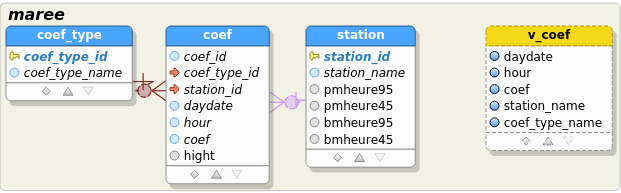
\includegraphics[width=0.8\textwidth]{../database/referentiel-maree}

Un script de génération de la base de données (\textit{create\_db.sql}) est fourni dans le dossier \textit{database}.
Si la structure est modifiée, il convient de modifier en conséquence les classes d'accès aux tables dans le dossier \textit{lib} : station.class.php pour la table des stations, et coef.class.php pour le stockage des coefficients de marée. 

\section{Exécution}
\subsection{Dépôt des fichiers}
Déposez les fichiers à traiter dans le dossier \textit{import}

\subsection{Lancement du script}

Linux :
\begin{itemize}
\item ouvrez un terminal, et positionnez-vous dans le dossier \textit{sonde}
\item la commande de lancement du script est sous la forme :
\begin{lstlisting}
php shomimport.php --options
\end{lstlisting}
\end{itemize}

Windows :
\begin{itemize}
\item Ouvrez un terminal \textit{PowerShell} (dans le menu, \textit{Windows PowerShell > Windows PowerShell})
\item Positionnez vous dans le sous-dossier \textit{magest} :
\begin{lstlisting}
cd .\Documents\shomimport
\end{lstlisting}
\item la commande de lancement du script est sous la forme (le chemin d'accès à \textit{php.exe} doit être adapté à la situation réelle) :
\begin{lstlisting}
../php/php.exe shomimport.php --options
\end{lstlisting}
\end{itemize}

\subsection{Options utilisables}

Plusieurs options peuvent être ajoutées à la ligne de commande. Elles vont surcharger les paramètres généraux du fichier \textit{param.ini}. Une seule est obligatoire : le nom de la station à traiter.

\begin{tabular}{|l|>{\raggedright\arraybackslash}p{12cm}|}
\hline 
Paramètre & Fonction \\ 
\hline 
station & nom de la station. Le nom est obligatoire, et une section portant ce nom doit exister dans le fichier de paramètres. De plus, le nom de la station doit exister dans la table \textit{station} de la base de données \\
dsn & Chaîne de connexion au serveur de base de données\\
login & Login utilisé \\
password & Mot de passe associé \\
schema & Nom du schéma contenant les données dans la base de données \\
source & Nom du dossier contenant les fichiers à traiter \\
treated & Nom du dossier où les fichiers seront déplacés après traitement \\
param & permet de charger un fichier autre que le fichier param.ini pour utiliser des paramètres spécifiques \\
filetype & extension des fichiers à traiter \\
noMove & Si vaut 1, les fichiers traités ne seront pas déplacés. \\
help & Le programme affiche un message récapitulant les options, puis s'arrête \\
\hline
\end{tabular}


\section{Copyright et assistance}
Le logiciel est sous Copyright © IRSTEA 2019. Il est distribué sous licence MIT.

Pour toute question ou suggestion, merci d'ouvrir un ticket dans la forge Github : \href{https://github.com/Irstea/shomimport/issues/new}{https://github.com/Irstea/shomimport/issues/new}
\end{document}